\chapter{Implementation, Pilot Results, and Future Work}
\label{Chapter4}

\begin{sloppypar}
This chapter presents the experimental implementation details, pilot benchmark evaluation results, clinician dashboard interface, and verification tests completed for the Mid-Semester milestone of Kent-AI. We then outline the immediate post-mid-semester roadmap and present conclusions.

\section{Implementation Status and Verified Deliverables}
At this mid-semester evaluation, the foundational and operational pipeline of Kent-AI is fully implemented across six distinct engineering phases, supported by \textbf{60 passing automated unit and integration tests} executed in 4.05 seconds under \texttt{pytest}.

\begin{table}[htp]
\centering
\caption{Mid-semester engineering deliverables and verification status.}
\label{tab:implementation_status}
\resizebox{\textwidth}{!}{%
\begin{tabular}{|l|l|l|c|}
\hline
\textbf{Phase} & \textbf{Module / Deliverable} & \textbf{Key Files} & \textbf{Status} \\
\hline
Phase 0 & Scaffolding \& SQLite DAL & \texttt{src/data/kent\_db.py} & \checkmark Complete \\
Phase 1 & Synthetic Generation Pipeline & \texttt{src/data/case\_generator.py} & \checkmark Pilot Benchmarked \\
Phase 2 & Dense ChromaDB Vector Store & \texttt{src/search/vector\_store.py} & \checkmark 74,513 Rubrics Indexed \\
Phase 4 & LLaMA 3 Negation Resolver & \texttt{src/models/resolver.py} & \checkmark Implemented \& Tested \\
Phase 5 & Kentian Totality Ranker & \texttt{src/search/ranker.py} & \checkmark Operational \\
Phase 6 & 10-State Intake Chatbot & \texttt{src/chatbot/state\_machine.py} & \checkmark Operational \\
Phase 7 & Clinician Dashboard Portal & \texttt{src/dashboard/app.py} & \checkmark Version 1 \\
\hline
\end{tabular}
}
\end{table}

\section{Dense Semantic Vector Store Performance (Phase 2)}
The full-scale indexing of Kent's Repertory into ChromaDB was executed on the developer workstation using \texttt{sentence-transformers/all-MiniLM-L6-v2}:
\begin{itemize}
    \item \textbf{Total Corpus Size}: 74,513 hierarchical rubric paths across all 37 sections.
    \item \textbf{Batch Indexing Duration}: Completed in \textbf{931.14 seconds} at an indexing throughput of \textbf{80.0 rubrics/second}.
    \item \textbf{Storage Format}: Persistent on-disk HNSW index (\texttt{data/embeddings/kent\_rubrics/}) requiring 384-dimensional unit-normalized float32 vectors.
    \item \textbf{Retrieval Latency}: Sub-15 millisecond cosine retrieval across all 74,513 vectors on CPU.
\end{itemize}

\subsection{Semantic Retrieval Verification Example}
A representative test query illustrates the system's ability to bridge the semantic divide:
\begin{itemize}
    \item \textbf{Query}: \emph{"splitting headache from sun exposure"}
    \item \textbf{Token Overlap with Repertory}: 0\% overlap on the root rubric terms.
    \item \textbf{Retrieved Top-3 Rubrics}:
    \begin{enumerate}
        \item \texttt{HEAD > PAIN > sun, from exposure to} (Similarity: 0.764 --- Strong Match)
        \item \texttt{HEAD > PAIN > bursting} (Similarity: 0.692 --- Strong Match)
        \item \texttt{HEAD > PAIN > pulsating > sun, from} (Similarity: 0.648 --- Good Match)
    \end{enumerate}
\end{itemize}

\section{Phase 1: Pilot Benchmark Evaluation (100 Stratified MIND Cases)}
To benchmark the synthetic case generation and 4-tier BIO auto-tagging pipeline, we generated and evaluated a pilot benchmark dataset of \textbf{100 clinical cases} distributed across \textbf{25 stratified MIND rubrics} (4 clinical archetypes per rubric) using local LLaMA~3 8B. The results are summarized in Table~\ref{tab:pilot_metrics}.

\begin{table}[htp]
\centering
\caption{Performance metrics on the 100-case pilot validation benchmark.}
\label{tab:pilot_metrics}
\resizebox{\textwidth}{!}{%
\begin{tabular}{|l|c|c|c|}
\hline
\textbf{Evaluation Metric} & \textbf{Achieved Result} & \textbf{Benchmark Target} & \textbf{Status} \\
\hline
\textbf{JSON Schema Validity} & \textbf{100.0\%} (100/100) & 100.0\% & \checkmark Passed \\
\textbf{BIO Character Offset Accuracy} & \textbf{100.0\%} (576/576 spans) & $\ge 98.0\%$ & \checkmark 0 Drift \\
\textbf{Token / Tag Sequence Alignment} & \textbf{100.0\%} (0 mismatches) & 100.0\% & \checkmark Passed \\
\textbf{Total Extracted Clinical Spans} & 576 spans (5.76/case) & $\ge 4.0$/case & \checkmark High Density \\
\textbf{Pairwise Jaccard Lexical Overlap} & \textbf{13.10\%} & $< 45.0\%$ & \checkmark Superior Diversity \\
\textbf{Lexical Diversity Score} & \textbf{86.90\%} & $> 55.0\%$ & \checkmark Non-Repetitive \\
\textbf{Average Token Length} & 73.1 tokens (range 34--131) & 50--120 tokens & \checkmark Optimal \\
\hline
\end{tabular}
}
\end{table}

\subsection{7-Dimension Entity Distribution}
The 576 extracted spans exhibit comprehensive coverage across Kent's dimensions:
\begin{itemize}
    \item \texttt{MENT} (Mental/Emotional): 286 spans (49.7\%)
    \item \texttt{SEN} (Sensation): 77 spans (13.4\%)
    \item \texttt{LOC} (Location): 76 spans (13.2\%)
    \item \texttt{MOD\_AGG} (Aggravation): 57 spans (9.9\%)
    \item \texttt{TEMP} (Temporal Modality): 39 spans (6.8\%)
    \item \texttt{CONC} (Concomitants): 34 spans (5.9\%)
    \item \texttt{MOD\_AMEL} (Amelioration): 7 spans (1.2\%)
\end{itemize}

\section{Doctor-Facing Clinical Dashboard}
Implemented in \texttt{src/dashboard/app.py}, the clinical dashboard adheres to the design system specification:
\begin{itemize}
    \item \textbf{Midnight Canvas Theme (\texttt{\#0A0F1D})}: High-contrast, dark-mode clinical UI featuring glassmorphic cards and glowing status telemetry.
    \item \textbf{Four Dedicated Workspaces}:
    \begin{enumerate}
        \item \emph{Live Consultation Workspace}: Real-time intake chat console with confined 450px scrolling container, live 7-dimension slot progress HUD, and dynamic suggestion chips.
        \item \emph{Instant Repertorization Workspace}: Interactive Totality Matrix grid mapping Candidate Remedies $\times$ Matched Rubrics with color-coded grade badges (Grade 3 Red/Crimson, Grade 2 Amber, Grade 1 Slate) and one-click Markdown/JSON report export.
        \item \emph{74k Rubric Tree Explorer}: Hierarchical navigation across all 37 sections with expandable 3-grade remedy inspectors.
        \item \emph{Materia Medica Keynote Index}: Rapid reverse-lookup displaying Grade 3 characteristic keynotes for any selected remedy.
    \end{enumerate}
    \item \textbf{Chapter 1 MIND Focus}: Configured with dedicated scoping for the 4,933 mental rubrics.
\end{itemize}

\begin{figure}[htp]
\centering
\textbf{(a) Live Clinical Consultation Workspace and Slot Tracking HUD}\par\smallskip
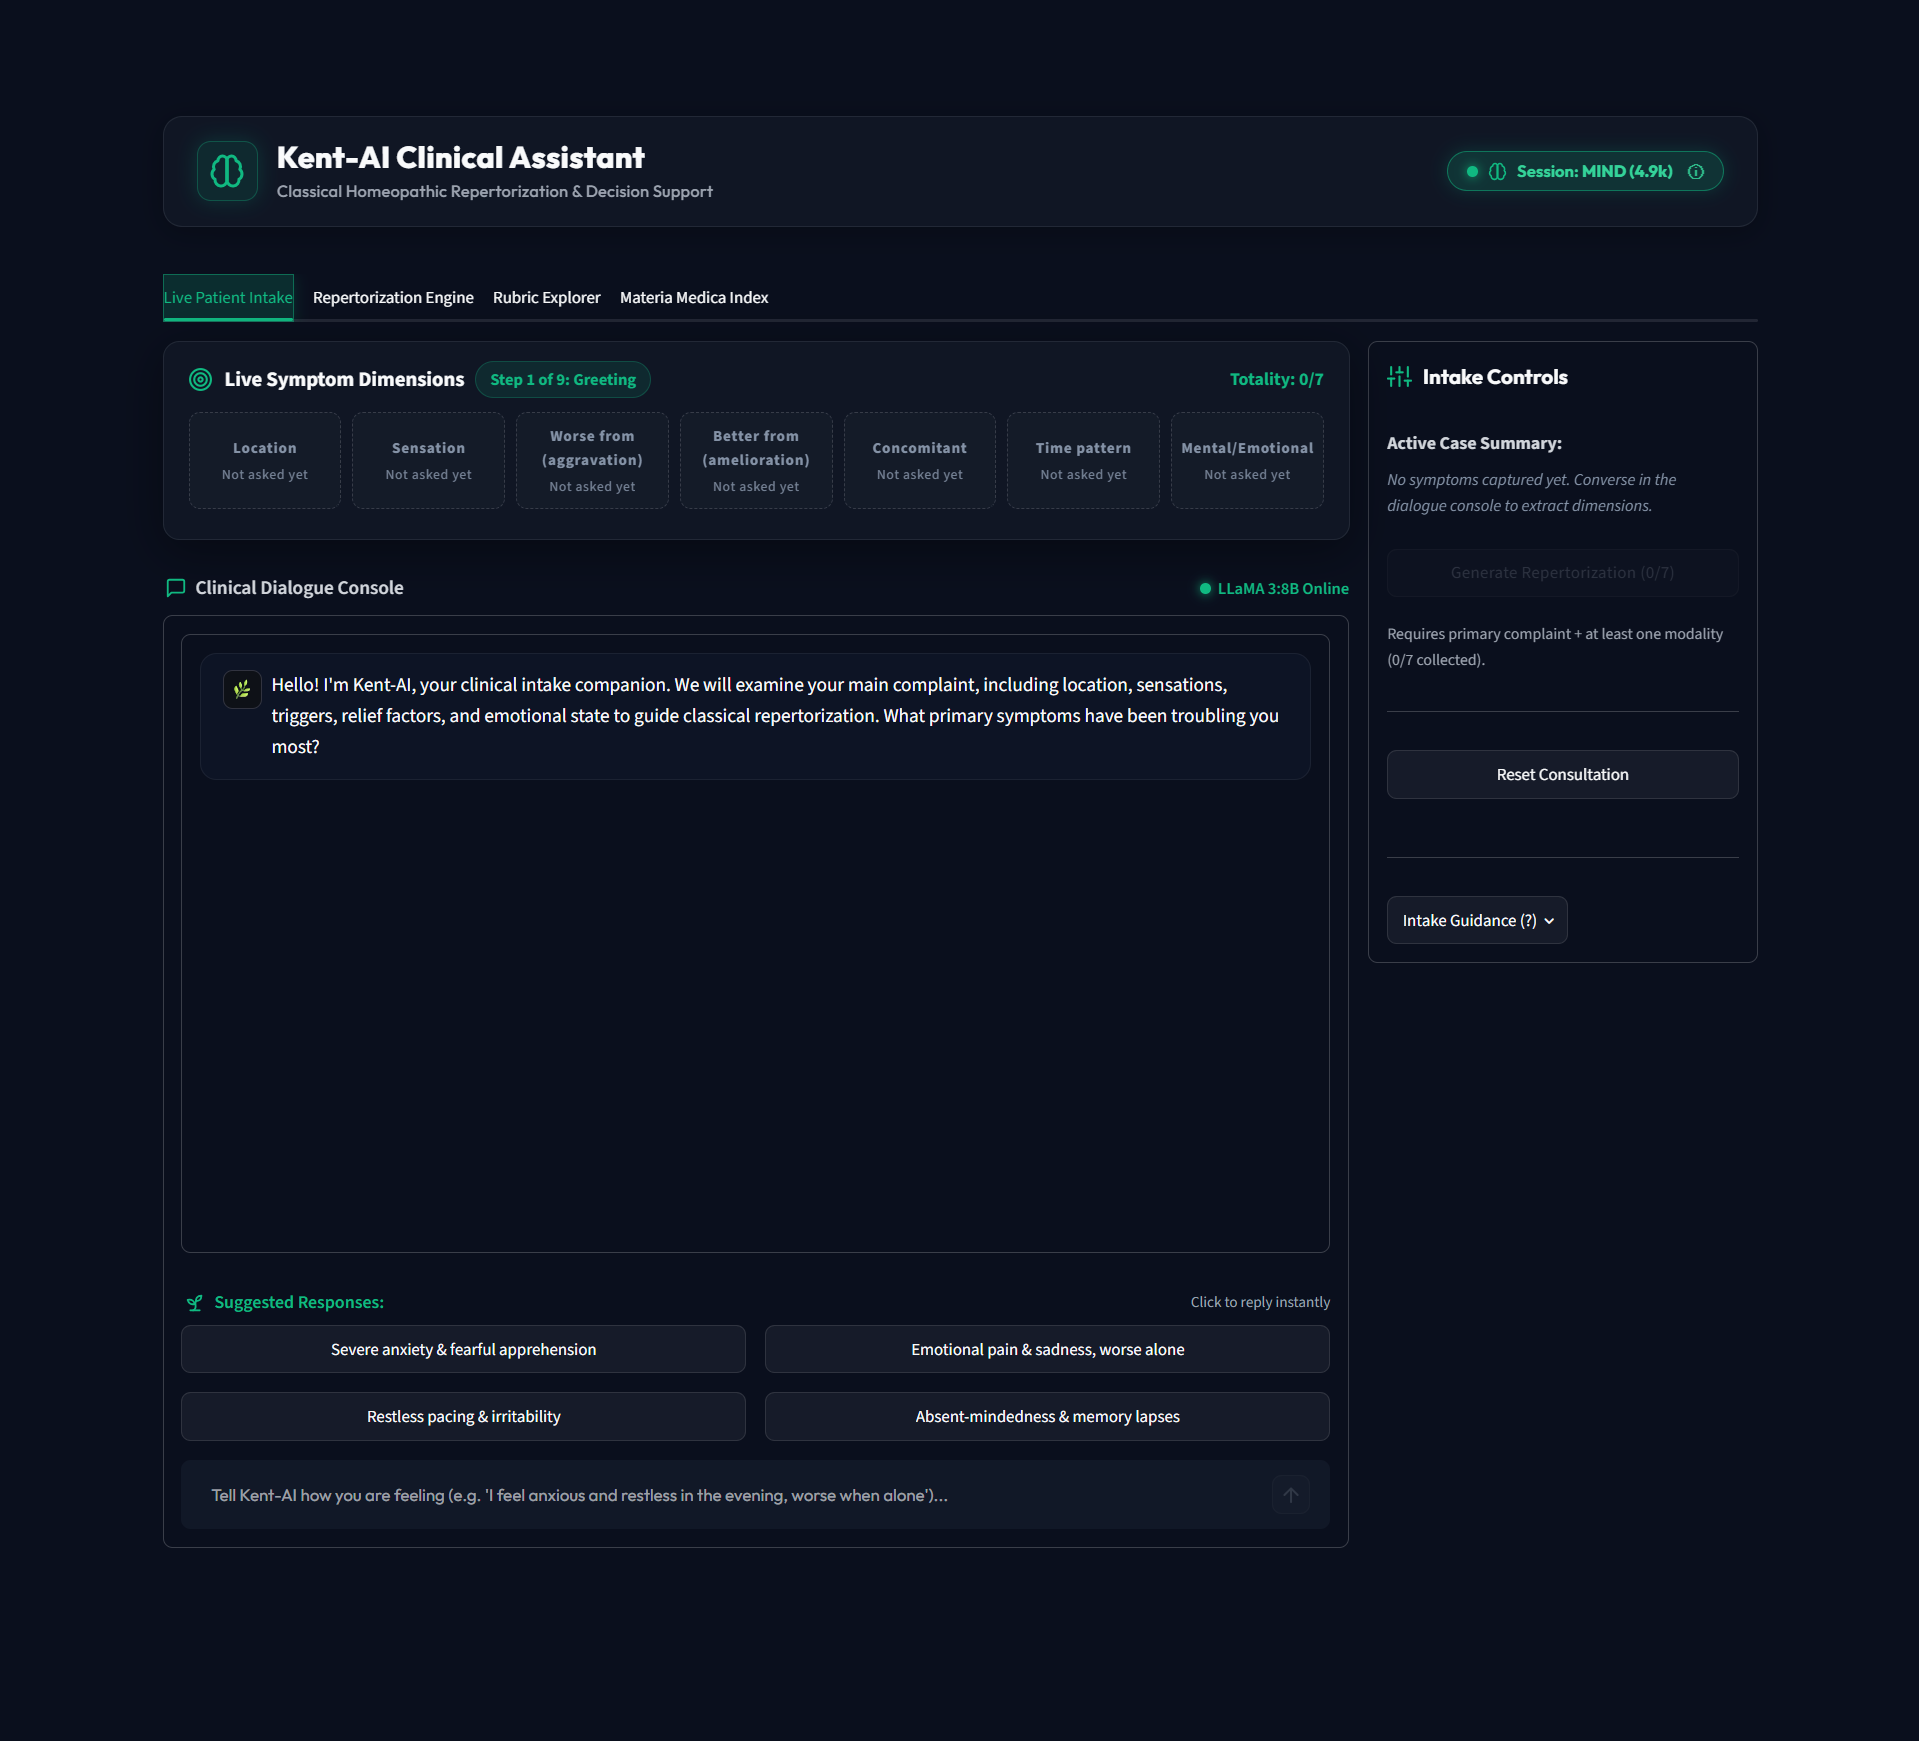
\includegraphics[width=0.88\textwidth]{Figures/dashboard_mockup.jpg}
\vspace{0.35cm}

\textbf{(b) Instant Repertorization Workspace and Remedy Totality Matrix}\par\smallskip
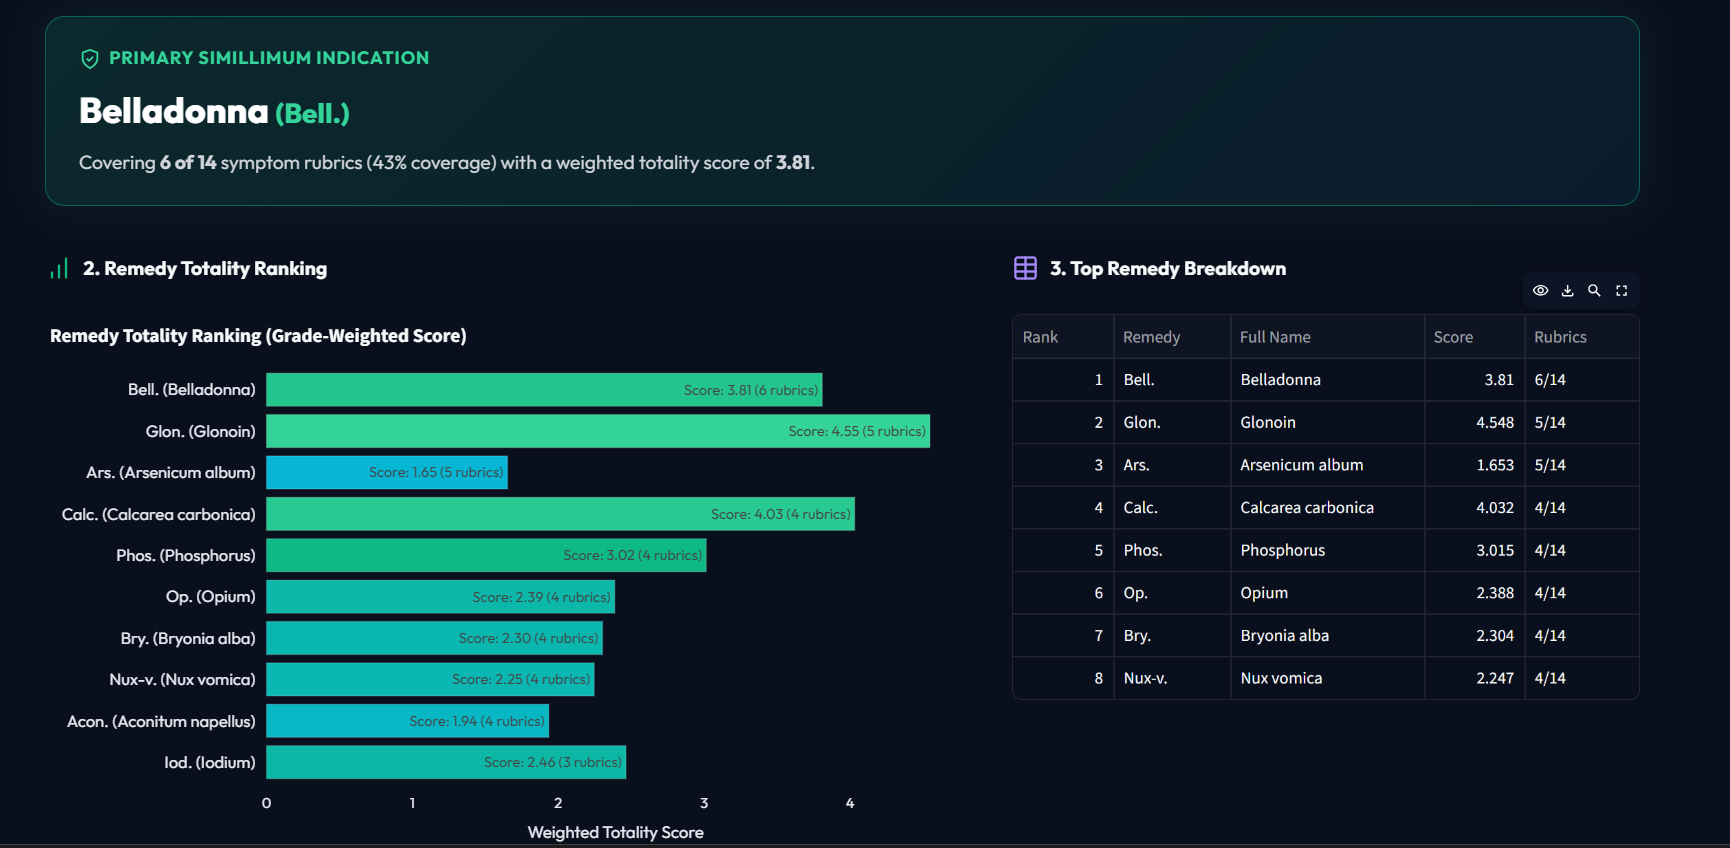
\includegraphics[width=0.88\textwidth]{Figures/dashboard_mockup-2-results.png}
\caption{Kent-AI doctor-facing clinical dashboard interface: (a) Live conversational intake console with real-time 7-dimension slot progress tracking and dynamic suggestion chips; (b) Instant repertorization workspace displaying candidate remedies against retrieved rubrics with 3-tier color-coded grades and one-click clinical report export.}
\label{fig:dashboard_ui}
\end{figure}

\section{Post-Mid-Semester Roadmap and Future Work}
Following the mid-semester evaluation, the project roadmap and future research directions focus on four key milestones:
\begin{enumerate}
    \item \textbf{Production Synthetic Case Generation}: Execute \texttt{scripts/run\_gpu\_generation.sh} on the departmental GPU cluster with atomic checkpoints, generating the full target corpus of \textbf{~22,200 synthetic clinical cases} across all 4,933 MIND rubrics (4 clinical variations/rubric) with stratified 80/10/10 deficit-balancing splits (\texttt{train.jsonl}, \texttt{val.jsonl}, \texttt{test.jsonl}).
    \item \textbf{Phase 3: Fine-Tuning \texttt{Bio\_ClinicalBERT}}: Train the token-level BIO sequence classifier on Google Colab T4 GPU over the generated training corpus, targeting Token-Level BIO F1 $\ge 88.0\%$.
    \item \textbf{Phase 5 \& 8: End-to-End Pipeline Evaluation and Quantitative Benchmarks}: Execute comprehensive pipeline evaluations on held-out test splits targeting Top-20 Rubric Recall $\ge 90.0\%$ and Mean Reciprocal Rank (MRR) $\ge 0.65$ across multi-symptom case scenarios.
    \item \textbf{Clinical Expert Validation with Homeopathy Practitioners}: To establish empirical validity beyond computational metrics, we will validate the Kent-AI tool in direct collaboration with certified homeopathic clinicians and domain experts. This clinical validation study will encompass:
    \begin{itemize}
        \item \emph{Prescription and Repertorization Validity}: Expert qualitative review of top-ranked candidate remedies against established Materia Medica keynotes and verified patient cure profiles to evaluate diagnostic fidelity.
        \item \emph{Rubric Concordance}: Expert evaluation of the dense semantic matcher's rubric mapping accuracy for complex, colloquial patient complaints.
        \item \emph{Consultation Time Reduction}: Controlled observational trials comparing conventional 30--45 minute case-taking sessions against Kent-AI-assisted consultations, validating the target reduction to under 10 minutes.
        \item \emph{Clinical Usability and Trust}: Assessment of practitioner trust, interpretability of the Kentian totality scoring breakdown, and overall dashboard workflow usability.
    \end{itemize}
\end{enumerate}

\section{Conclusion}
Kent-AI successfully bridges the gap between 19th-century classical homeopathic literature and 21st-century neural natural language processing. By combining an empathetic 10-state conversational intake FSM, token-level clinical entity recognition, dense semantic vector retrieval over 74,513 rubrics in ChromaDB, and a transparent Kentian totality scoring engine, Kent-AI resolves the critical clinical bottlenecks of case-taking time, cognitive fatigue, and vocabulary mismatch. The mid-semester implementation stands verified with 60 passing tests and a 100-case pilot benchmark, establishing a solid foundation for final model fine-tuning, system evaluation, and clinical validation with practicing homeopathic experts.

\end{sloppypar}
